%% Example of a LaTeX source file for a COLING-2012 submission
%% last updated: July 10, 2012
%% Optional instructions for authors within the tex file are provided as comments and start with 'for authors:...'
\documentclass[10pt,a5paper,twoside]{article}
\usepackage{coling2012}
\title{Article Title: document template for COLING-2012}
%for authors: in case of more than four author names ref. to commented line below 
%\author{$Annie~SMITH^{1, 2}~~~LI~Xiao Dong^{1, 3}$\\$~~~Third~Author^{1, 2}~~~Fourth~Author^{1, 3}~~~ Fifth~Author^{2, 3}$\\
\author{$Annie~SMITH^{1, 2}~~~LI~Xiao Dong^{1, 3}$\\
{\small  	(1) INSTITUTE\_1, address 1\\ 
 		(2) INSTITUTE\_2, address 2\\
		(3) INSTITUTE\_3, address 3\\
  \texttt{Annie.Smith@institute.edu.ca, Li.Xiao-Dong@iitb.ac.in} \\ 
}}

\begin{document}
\maketitle
%% The first mandatory ABSTRACT (\abstractEn) section below is for the English language
\abstractEn{  %ABSTRACT}{
Place for the abstract in English (maximum 150 words). \\	
This is a template for the submissions and proceedings of COLING-2012 and associated events. The Programme Committee and the Organizing Committee want to encourage participants to read as many contributions as possible during the conference and the workshops, and to lower the number of copies and the unit cost of paper proceedings. To ensure very good readability on PC screens as well as good readability of the paper in proceedings, authors are encouraged to use the \emph{Charter} font (for LaTeX) and the \emph{Charis} or \emph{Georgia} font (for MS or Libre Office word processors) if they can, otherwise please use \emph{Times New Roman}. Also, \emph{the format will be A5} (2 pages on screen, 1 page on a larger standard format in print). The title of the article is in 14pt, bold, centered. Authors are in italics, 11pt, centered; affiliations in 9pt.  E-mail addresses are in Courier New, 10pt, centered.}

%for authors: the line below is for instruction purposes and can be commented
\textbf{AT SUBMISSION TIME, PLEASE ANONYMISE everywhere, REPLACING NAMES BY DUMMIES LIKE John DOE\_1, Jack DOE\_2.}

%for authors: the abstract section below is optional and can be commented otherwise
%% The second ABSTRACT (\abstractOL) given below is for the optional language
\abstractOL{ %TITLE AND ABSTRACT IN ANOTHER LANGUAGE, $L_{2}$ (OPTIONAL, AND ON SAME PAGE)}{
\\\\
{\centering{{\Large{\textbf{Translation in $L_{2}$ of the article title}}} (if option used):14pt, bold,centered}}\\\\
The translation of the title and abstract in another language $L_{2}$ is optional.  If the title is translated, the abstract must also be translated, as exactly as possible. In that case, put an abstract in $L_{2}$ (maximum 170 words as translation expands text length) here.\\\\
Apart from enhancing visibility in one’s own national scientific communities, these parallel abstracts might be the seed for a multilingual natural parallel corpus in computational linguistics.
Tantus est igitur innatus in nobis cognitionis amor et scientiae ut nemo dubitare possit quin ad eas res hominum natura nullo emolumento invitata rapiatur. Videmusne ut pueri ne verberibus quidem a contemplandis rebus perquirendisque deterreantur ? Ut pulsi recurrant? Ut aliquid scire se gaudeant ? Ut id aliis narrare gestiant ? Ut pompa, ludis atque eius modi spectaculis teneantur ob eamque rem vel famem et sitim perferant ? Quid vero ? 
}

%%-------------
%for authors: if only English language option is chosen comment the \abstractOL section above and use \keywordsEn below 
%for authors: else use add title and abstract to \abstractOL section above and use \keywordsOL below (case-sensitive commands)

%for authors: for keywords section either use \keywordsEn OR \keywordsOL below as relevant
%Example for English only keywords list
%\keywordsEn{Here a list of keywords in English}

%Example for English + optional language keywords list
\keywordsOL{Here a list of keywords in English}
{Here a list of keywords in $L_{2}$ (if option used)}
%%--------------

\newpage
%================================================================
% section 1
\section{Optional condensed 2-page version in $L_{2}$ (1st section if present)}
If the “other language” option is used on the first page, it is possible to put here a condensed version of the paper in the same L2 language. It should take no more than 2 pages.\\
The remaining of this section is not an example of a condensed version, rather a quick experiment to translate the above sentence with 2 widely known MT systems (PE below means  PostEditing).
 
 \begin{longtable}{|l|l|p{10.5cm}|}
 \hline
 FR  &~~ Google  & Si le "autre langue" option est utilis\'ee sur la premi\`ere page, il est possible de mettre ici une version condens\'ee du papier dans la m\^eme langue $L_{2}$. Il ne devrait pas prendre plus de 2 pages.   \\
 \hline
   &~~ Systran  & Si l'option de la " autre langue " est employ\'ee \`a la premi\`ere page, il est possible de mettre ici une version condens\'ee du papier dans la m\^eme langue $L_{2}$. Il devrait ne prendre pas plus de 2 pages.  \\
 \hline
   &~~ PE  & Si l'option " autre langue " est employ\'ee \`a la premi\`ere page, il est possible de mettre ici une version condens\'ee du papier dans la m\^eme langue $L_{2}$. Cela devrait ne prendre pas plus de 2 pages.  \\
 \hline
 DE  &~~ Google  & Wenn die "andere Sprache" Option auf der ersten Seite verwendet wird, ist es m\"oglich, hier legte eine gek\"urzte Fassung des Papiers in der gleichen Sprache $L_{2}$. Es sollte nicht mehr als 2 Seiten.  \\
 \hline
   &~~ Systran  & Wenn die "andere Sprach" Wahl auf der ersten Seite verwendet wird, ist es m\"oglich, eine verk\"urzte Version des Papiers in die gleiche Sprache $L_{2}$ hier einzusetzen. Es sollte nicht mehr als 2 Seiten nehmen.  \\
 \hline
   &~~ PE  & Wenn die "andere Sprache" Wahl auf der ersten Seite verwendet wird, ist es m\"oglich, eine verk\"urzte Version des Berichts in der gleichen Sprache $L_{2}$ hier einzusetzen. Es sollte nicht mehr als 2 Seiten einnehmen.  \\
 \hline
 ZH  &~~ Google  & ZH content could be entered using native language support packages (if available) \\
 \hline
   &~~ Systran  & ZH content could be entered using native language support packages (if available) \\
 \hline
   &~~ PE  & ZH content could be entered using native language support packages (if available) \\
 \hline
 RU  &~~ Google  & RU content could be entered using native language support packages (if available) \\
 \hline
   &~~ Systran  & RU content could be entered using native language support packages (if available) \\
 \hline
   &~~ PE  & RU content could be entered using native language support packages (if available) \\
 \hline
 GR  &~~ Google  & GR content could be entered using native language support packages (if available) \\
 \hline
   &~~ Systran  & GR content could be entered using native language support packages (if available) \\
\hline
   &~~ PE  & GR content could be entered using native language support packages (if available) \\
\hline
JP  &~~ Google  & JP content could be entered using native language support packages (if available) \\
 \hline
   &~~ Systran  & JP content could be entered using native language support packages (if available) \\
 \hline
   &~~ PE  & JP content could be entered using native language support packages (if available) \\
 \hline
AR  &~~ Google  & AR content could be entered using native language support packages (if available) \\
 \hline
  &~~ Systran  & AR content could be entered using native language support packages (if available) \\
 \hline
KR  &~~ Google  & KR content could be entered using native language support packages (if available) \\
 \hline
  &~~ Systran  & KR content could be entered using native language support packages (if available)  \\
\hline
ES  &~~ Google  & Si el "otro idioma" opci\'on se utiliza en la primera p\'agina, es posible poner aqu\'i una versi\'on resumida del documento en el mismo lenguaje L$_{2}$. Se debe tener no m\'as de 2 p\'aginas.  \\
 \hline
   &~~ Systran  & Si la opci\'on de la "otra lengua" se utiliza en la primera p\'agina, es posible poner aqu\'i una versi\'on condensada del papel en la misma lengua L$_{2}$. Debe tomar no m\'as que 2 p\'aginas.  \\
 \hline
   &~~ PE   & Si la opci\'on "otra lengua" se utiliza en la primera p\'agina, es posible poner aqu\'i una versi\'on condensada del papel en la misma lengua L$_{2}$. Debe tomar no m\'as que 2 p\'aginas.\\
 \hline
PR  &~~ Google  & Se o "outro idioma" op\c{c}\~ao \'e usada na primeira p\'agina, \'e possível colocar aqui uma vers\~ao condensada do papel na língua L$_{2}$ mesmo. Deve ter no m\'aximo 2 p\'aginas. \\
\hline
  &~~ Systran  & Se da "a op\c{c}\~ao outra l\'ingua" \'e usada na primeira p\'agina, \'e poss\'ivel p\^or aqui uma vers\~ao condensada do papel na mesma l\'ingua L$_{2}$. Deve tomar n\~ao mais de 2 p\'aginas.  \\
\hline
IT  &~~ Google  & Se l ' "altro linguaggio" opzione viene utilizzata nella prima pagina, \'e possibile mettere qui una versione condensata della carta nella stessa lingua L$_{2}$. Essa non dovrebbe richiedere pi\`u di 2 pagine.  \\
\hline
  &~~ Systran  & Se " l'opzione dell ' altra lingua" \`e usata alla prima pagina, \`e possibile mettere qui una versione condensata della carta nella stessa lingua L${_2}$. Dovrebbe prendere non non pi\`u di 2 pagine.  \\
\hline
  &~~ PE  & Se l'opzione "altra lingua" \`e usata alla prima pagina, \`e possibile mettere qui una versione condensata del articolo nella stessa lingua L$_{2}$. Dovrebbe prendere non pi\`u di 2 pagine. \\
\hline 
HI  &~~ Google  & HI content could be entered using native language support packages (if available) \\
\hline
   &~~ Systran  & HI content could be entered using native language support packages (if available) \\
 \hline
   &~~ PE  & HI content could be entered using native language support packages (if available) \\
 \hline 
\end{longtable} 
 Urdu, Tamil and other languages don't display well at this moment (our fonts are not complete).
 \newpage

% section 2
\section{Main content of the paper (in English)}
% subsection 2.1
\subsection{General information}
This template continues as if the "other language" option had been chosen, meaning that the article proper, in English, begins on page 4. Its length corresponds to that of a short paper.

USUAL but IMPORTANT: papers must conform to the official COLING-2012 style guidelines (downloadable from the website).

Submission and reviewing will be on-line, managed by the START system. The only accepted format for submitted papers is PDF. Supplementary material, if any, in the form of tools or resources, must be in the form of a single .zip or a .tgz archive file with a maximum size of 10MB; otherwise there are no constraints on its format. Submissions, together with all supplementary material, must be uploaded on the START system by the submission deadlines; submissions after that time will not be reviewed.

To minimize network congestion, we request authors to upload their submissions as early as possible (especially if they contain large supplementary material files). Improved versions of the submissions may be uploaded until the deadline.

Submissions must be in the format described in this template. If for some reason you have a problem producing this format, please contact organisers as early as possible. Organisers reserve the right not to publish papers not conforming to the required format.

On acceptance of a submission, precise instructions will be given on how to send the camera ready version, and in some cases with required modifications. Camera ready versions not conforming to programme committee’s improvement requests will be considered as unsent, and hence will not be presented at the conference and will not be included in the proceedings.
% subsection 2.2
\subsection{More on the format of submissions}
Since several years, scientific conferences have been distributing proceedings on electronic media to avoid producing printed versions. Printed versions are given to only those participants who explicitly request and pay for them. Most participants get the proceedings on a CD or on a USB key. That is a very good idea, but the drawback is that very few participants manage to read more than a small number of papers, typically less than 1/10th or 1/20th of the number available in the proceedings. The main reason seems to be that is it very awkward to read traditional A4 sized portrait double-column articles on usual laptop screens. 

The recent JEP-TALN-RECITAL-2012 conferences have successfully addressed that problem by proposing a template that is optimised for reading on PC screens. COLING-2012 and associated events propose to use it, with the option of using the Times New Roman font for authors having problems with installing the slightly better fonts Charter, Charis, or Georgia. 

%% below commented section for testing font sizes ---------
%\\{\small text with small style}\\
%line formatted with default font style equal normalsize (and is10pt; as defined in the \documentclass)\\
%{\normalsize text with normalsize style, \textbf {More on the format of submissions}}\\
%{\large text with large style, \textbf {More on the format of submissions}}\\
%{\Large text with Large style, \textbf {More on the format of submissions}}\\
%% end font size testing -----------
-
% 2.2.1
\subsubsection{Document format \& character fonts}
\emph{Submissions will be in PDF, with page dimensions of 150 mm x 210 mm, and margins of 5 mm on all sides.} That corresponds to A5 (148.2 mm x 209.9 mm) with 4.1 mm horizontal margins and 5 mm vertical margins.  To get the same layout on an A4 format while preparing a submission, choose A4 and put the margins at 35 mm (horizontal) and 48.3 mm (vertical).
\newpage
\emph{No header or footer should be present in submissions.}

The \emph{preferred fonts} have been chosen because they are optimised for reading on screen while being elegant in print. If possible, submissions prepared with LaTeX should use the \emph{Charter (Bitstream)} font. Users of Word or LibreOffice should use an equivalent font, namely (in order of preference):
\begin{compactenum}
\item\emph{Charter} (via Bitstream), available on most Linux and in LaTeX \emph{texlive} installations.
\item\emph{Charis SIL} (via SIL). It is an extension of the Charter font, and is available at \href{http://scripts.sil.org/cms/scripts/page.php?item_id=CharisSIL_download}
{http://scripts.sil.org/cms/scripts/page.php?item\_id=CharisSIL\_download}); 
\item\emph{Georgia.} This font is included  in MS Word by default.
\end{compactenum} 
If authors encounter problems in installing one of the preferred fonts, they should use Times New Roman (available in all platforms) as default font, with the same point sizes.

\emph{The body of the text should be in size 10pt, the titles in bold 11pt for levels 1 \& 2, and 10pt from level 3 onwards.}
%2.2.2
\subsubsection{Pages and paragraphs}
Paragraphs use single spacing and are justified left and right. They are not indented, but are separated by a half-line vertical space (6pt above and below).

The first page contains only the title, the names and affiliations of authors, the abstract(s) and the keywords (see page 1 of this template).

The body of the paper, including the introduction, begins on page 4 if a condensed (2-page) synopsis in another language L$_{2}$ is included, and on page 2 otherwise. 

A LaTeX stylesheet, a Word template, and an ODT template are available on the COLING-2012 website. Submissions will be handled interactively under SoftConf. 
%2.2.3
\subsubsection{Submission sizes}
Here are the length limits according to the type of submission. "Any number of reference pages" means that pages used for bibliographical and Internet references are not counted in the page number limits. However, it stands to reason that reviewers will accept only reasonable sizes.\\\\\\
\begin{tabular}{|l|l|l|}
\hline
full papers & 14 A5 pages with any number of reference pages & Oral presentation\\
\hline
short papers & 8 A5 pages with any number of reference pages & Poster presentation\\
\hline
demo papers & 6 A5 pages with any number of reference pages & Demonstration\\
\hline
\end{tabular}\\

Papers are in English. However, if an author so wishes s/he may add elements in another language (L$_{2}$): a title, an abstract and keywords on the first page, and 2 pages (a synopsis) in L$_{2}$, beginning on page 2. Such papers will have 14+2 (or 8+2, or 6+2) pages, plus any number of pages for reference. 
%2.3
\subsection{Other formatting elements}
%2.3.1	
\subsubsection{Lists}
Here is a bulleted list, where each element begins with an independent sentence (capitalized).
\begin{compactitem}
\item Its lines are separated by less vertical space than normal paragraphs.
\item We don’t add space between paragraphs of that same style.
\end{compactitem}

Here is a numbered list of items that are parts of an outside sentence. Take care to:
\begin{compactenum}
\item restart the numbering and get the numbers consecutive. 
\item not to capitalize the initial letter of such items.
\end{compactenum}
%2.3.2
\subsubsection{Figures and tables}
Figures and tables will be centered on the page, with a caption underneath. The caption will contain the keyword \textsc{Figure} or \textsc{Table} in small capitals, followed by the number of the figure or table. Numbers in each category are independent. Examples appear in this template. Equations and formulae may appear in line or centered on the page, without captions. A reference number may appear to the right of a formula or an equation.

\begin{table}[!h]
\setcounter{table}{0}
\centering
	\begin{tabular}{|c|p{5cm}|}
	\hline
	A table&\\
	\hline
	&The table is centered. Its cells may be optionally centered. Avoid full justification leading to very long horizontal spaces.\\
	\hline
	\end{tabular}
\caption{A table caption appears under it.}\label{Table}
\end{table}
%2.3.3
\subsubsection{Notes and references}
Footnotes\footnote{Here is one!} can be used.

References to the bibliography, for example \cite{Bernhard07}, are formatted with the APA style (see \href{http://www.apastyle.org/}{http://www.apastyle.org/}). It is available in all the LaTeX installations based on \emph{texlive} and on CTAN.

Users of Word or LibreOffice are encouraged to follow this style as much as possible when using their bibliography management tool (Mendeley, Zotero or Endnote). They can refer to the example below. Authors citing online references (URLs) should include the creation date in the reference.

The rest of this document only illustrates the format described above.

Tantus est igitur innatus in nobis cognitionis amor et scientiae ut nemo dubitare possit quin ad eas res hominum natura nullo emolumento invitata rapiatur. Videmusne ut pueri ne verberibus quidem a contemplandis rebus perquirendisque deterreantur ? Ut pulsi recurrant? Ut aliquid scire se gaudeant ? Ut id aliis narrare gestiant ? Ut pompa, ludis atque eius modi spectaculis teneantur ob eamque rem vel famem et sitim perferant ? Quid vero ? Qui ingeniis studiis atque artibus delectantur, nonne videmus eos nec valetudinis nec rei familiaris habere rationem omniaque perpeti ipsa cognitione et scientia captos et cum maximis curis et laboribus compensare eam quam ex discendo capiant voluptatem ?
\newpage
\begin{figure}[htbp] 
\begin{center}

\includegraphics[scale=0.70]{coling_logo.jpg}
\caption{An image used as a figure: It is a good idea to put each figure in a table cell to avoid (in Word) problems with anchored or floating figures.}
\label{image} %
\end{center} 
\end{figure} %
Omne hoc tempus inter pugillares ac libellos iucundissima quiete transmisi. "Quem ad modum, inquis, in urbe potuisti ?"

Circenses erant, quo genere spectaculi ne levissime quidem teneor. nihil novum, nihil varium, nihil quod non semel spectasse sufficiat. Quo magis miror tot milia virorum tam pueriliter identidem cupere currentis equos, insistentis curribus homines videre.

Si tamen aut velocitate equorum aut hominum arte traherentur, esset ratio non nulla; nunc favent panno, pannum amant, et, si in ipso cursu medioque certamine hic color illuc, ille huc transferatur, studium favorque transibit, et repente agitatores illos, equos illos, quos procul noscitant, quorum clamitant nomina, relinquent. Tanta gratia, tanta auctoritas in una vilissima tunica, mitto apud volgus, quod vilius tunica, sed apud quosdam graves homines; quos ego cum recordor in re inani, frigida, assidua tam insatiabiliter desidere, capio aliquam voluptatem, quod hac voluptate non capior.

Ac per hos dies libentissime otium meum in litteris colloco, quos alii otiosissimis occupationibus perdunt. Vale. (PLINE Junior, Letters, IX, 6.) 
\begin{figure}[htbp]
\begin{center} 
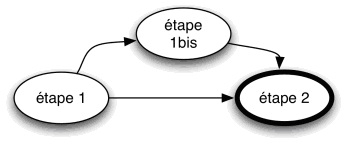
\includegraphics[scale=0.4]{illustration2.jpg} 
\caption{It is not advised to use Word directly to generate drawings. Use another tool (even Powerpoint) and insert the resulting image (at least 300 DPI or in vectorised format).}
\label{figure}
\end{center}
\end{figure} 

%3
\section{Title of a section}
Rem atrocem nec tantum epistola dignam Larcius Macedo, vir praetorius, a servis suis passus est, superbus alioqui dominus et saevus et qui servisse patrem suum parum, immo nimium meminisset. Lavabatur in villa Formiana; repente eum servi circumsistunt, alius fauces invadit, alius os verberat, alius pectus et ventrem atque etiam, foedum dictu, verenda contundit; et, cum exanimem putarent, abiciunt in fervens pavimentum, ut experirentur an viveret. 

Ille, sive quia non sentiebat, sive quia non sentire se simulabat, immobilis et extentus fidem peractae mortis implevit. Tum demum quasi aestu solutus effertur; excipiunt servi fideliores, concubinae cum ululatu et clamore concurrunt. Ita et vocibus excitatus et recreatus loci frigore, sublatis oculis agitatoque corpore vivere se - et iam tutum erat - confitetur. \\
\newpage
Diffugiunt servi quorum magna pars comprehensa est, ceteri requiruntur; ipse paucis diebus aegre focilatus non sine ultionis solacio decessit, ita vivus vindicatus ut occisi solent. (PLINE, Letters, III, 14.)
%3.1	
\subsection{Title of a subsection}
Miles cum oboediens potestati, sub qua legitime constitutus est, hominem occidit, nulla civitatis suae lege reus est homicidii; immo, nisi fecerit, reus est imperii deserti atque contempti. Quod si sua sponte atque auctoritate fecisset, in crimen effusi humani sanguinis incidisset. Itaque unde punitur si fecit iniussus, inde punietur nisi fecerit iussus. Quod si ita est, iubente imperatore, quanto magis, iubente creatore ! 
%3.1.1
\subsubsection{Title of a subsubsection}
Qui ergo audit non licere se occidere, faciat, si iussit cuius non licet iussa contemnere; tantummodo videat utrum divina iussio nullo nutet incerto... Hoc dicimus, hoc asserimus, hoc modis omnibus approbamus neminem spontaneam mortem sibi inferre debere velut fugiendo molestias temporales, ne incidat in perpetuas. (Sanctus Augustinus.)

\section*{Conclusion and perspectives (not numbered, use style “Heading1”)} %  not numbered
This section should better not be numbered (style “Heading1” inherits from “Heading 1”).
\section*{Acknowledgments (not numbered, use style Heading1)}
Optional section. If some named entities may lead to authors identification, please anonymize them.	\\
Thanks to Gilles S\'erasset for having kindly shared with us the templates he devised for TALN-JEP-RECITAL-2012. 

%'apalike-fr' style below applies smallcaps style on author names
%in order to apply 'apalike-fr' the babel package must be given [frenchb] option instead of [english]
% \usepackage[frenchb]{babel} also causes title "References" to render with French accents like "R\'ef\'erences"
%\bibliographystyle{apalike-fr}

%'apa' style does not apply "smallcaps style" on author names and goes with the [english] option in the babel package

\bibliographystyle{apa}

\bibliography{colingbiblio}
\nocite{TALN2007,LaigneletRioult09,LanglaisPatry07,au1972,cks1981,mb2012}

%%================================================================
\end{document}
